\chapter{Introduction}
\label{ch:introduction}

This thesis presents measurements of events with
three leptons, two forward ``jets'' of clustered hadronic particles,
and an imbalance of transverse momentum
produced in proton-proton (\pp) collisions at the Large Hadron Collider (LHC).
Events are selected to isolate contributions involving the simultaneous
production of a $\PW^{+}$ or $\PW^{-}$ and a $\PZ$ boson, the heavy particles
that communicate the weak force.
Selected events are used
to measure the rate of production of processes predicted by the standard
model (SM) of particle physics, the most complete theoretical expression
of the known particles and forces of the universe, and to search for hypothetical extension
of the SM. 

A dedicated search
for a rare, previously unobserved SM process, referred to as electroweak (EW)
WZ (\EWWZ) production, is presented. 
The presence and production rate of the \EWWZ process is intimately connected to the 
structure of the weak interaction and the 
phenomenon of EW symmetry breaking (EWSB) \cite{Quigg:2009vq}, which leads to 
the {\PW} and {\PZ} bosons acquiring mass.
A fundamental prediction
of EWSB, fulfilled in the standard model (SM) by the Brout-Englert-Higgs (BEH) 
mechanism~\cite{PhysRevLett.13.321,Higgs:1964ia,PhysRevLett.13.508,PhysRevLett.13.585,PhysRev.145.1156,PhysRev.155.1554}. 
is the emergence of a scalar particle, known 
to as the Higgs boson. 
This particle was first observed by the 
ATLAS~\cite{Aad:2012tfa} and CMS~\cite{Chatrchyan:2012xdj,Chatrchyan:2013lba} Collaborations
at CERN in 2012, providing compelling evidence for the BEH mechanism as
a component of the SM theory.
This is the first study of this process performed by the CMS Collaboration.
Selected events are used to place constraints on physics beyond the SM (BSM) in terms
of explicit models predicting charged Higgs bosons, decaying to a $\Wpm$ and a $\PZ$
boson, and on generalized models of new interactions modifying
in the rate of production, or in kinematic distributions, of selected events.

\section{The universe of particles}

The idea of understanding the physical world by identifying its
fundamental constituents is a very old one. Ancient eastern and
western philosophers independently attempted the feat, concluding
that the world could be reduced 
to ``elements'' such as water, earth, and fire.
As observational science became a more prominent component of modern thought, 
evidence mounted that these elements themselves were 
not indivisible. Perhaps the Greeks had not identified
the correct fundamental elements, but the belief that this endeavor could
be accomplished lived on.

A major attraction of identifying the fundamental building blocks of the universe
is the implication for constructing a macroscopic description from these
pieces. This process of understanding a complex system 
by reducing it to its essential components
termed ``reductionism'' by philosophers, 
has formed the backbone of scientific endeavor for much of history.
In practice, the step from the fundamental to the macroscopic 
is far from trivial. Despite a well-established
understanding of the proton constituents and their interactions,
predicting the proton mass from first principles has only recently 
been achieved~\cite{Durr:2008zz}, and larger systems remain well
out of reach.
In addition to the challenges of calculability, additional structures
may arise from the nature of large systems, such as ferromagnetism or 
superconductivity.
This long-accepted path to a complete description of the physical world
has thus been called into question, and it may never be feasible
to achieve a theory of biology built from the findings of particle 
physics~\cite{Anderson393}.
Yet there is an undeniable elegance in achieving a concise description
of the fundamental elements of the natural world and their interactions,
and this remains the target of the field of particle physics today. 

The modern genesis of the field can perhaps be credited to 
the discovery of the electron in 1897 by J. J. Thomson, a particle still
believed to be elementary today~\cite{}.
Further experiments showed that the electron carries the smallest quantity of electric charge found
freely in nature, and we now know that many macroscopic electrical phenomena
arise from the motion of electrons in atoms.
A mathematical understanding of these electromagnetic interactions had 
already been established by James Clerk Maxwell decades before Thompson's work.


The idea of a particle of light is therefore seemingly at odds with Maxwell's theory,
which described light as a oscillations of electromagnetic fields,
but a quanta of light was central to the explanation of black-body radiation provided by Max Planck 
and for the theoretical explanation of the photoelectric effect developed by Albert Einstein.
The theory of fields and particle-like characteristics of electromagnetic
interactions were reconciled shortly after these proposals by the 
rapidly-developing quantum theory.
The quanta of light, the photon, is now understood to communicate the electromagnetic force.
By the early 1940s, these pieces had evolved into the theory of quantum 
electrodynamics, the first
quantized theory of particles and their interactions in the language 
of quantum field theory. 

Simultaneous to the efforts to develop a mathematical language to describe 
the fundamental particles and their interactions was an experimental effort 
to find and categorize them. New equipment for detecting these particles,
such as the cloud chamber developed by Charles Wilson~\cite{}, 
gave a perspective on the spontaneous 
decay of atoms and opened our eyes to the radiation bombarding the earth from
outside the atmosphere. By the 1950s, particle physicists were faced with a ``particle zoo''
of seemingly fundamental objects spanning a huge range of masses. 
An underlying structure of the properties of many of these particles, 
now known as hadrons, was described by Murray Gell-Man and George Zweig in 1964.
They realized the properties of the many observed hadrons could be 
attributed to combinations of different elementary particles,
which Gell-Man termed quarks.
Whether these particles were physical entities or abstractions was 
not immediately evident, but experiments at the Stanford Linear Accelerator
at the end of the 1960s showed the proton to have point-like constituents
with the properties Gell-Man and Zweig predicted.

Despite the progress in explaining the structure of hadronic matter,
it remained unclear that the language of a quantum gauge theory, 
so successful in the formulation of the electromagnetic interaction, could 
also describe the strong nuclear force responsible for the formation
of these composite particles, and the weak nuclear force responsible for
a subset of their decays. Both exhibited striking differences with
respect to the electromagnetic interaction:
the weak nuclear force acts over a much smaller distance, while
the strong nuclear 
force has an inverted scaling with distance, increasing at higher separation
of the interacting objects while decreasing at very short ranges. 

A unification of the electromagnetic and weak nuclear force was achieved
by Sheldon Glashow, Abdus Salam, and Steven Weinberg in the early 1970s.
A crucial component of their theory is the presence of a scalar field, 
which gives mass to the W and Z bosons through EWSB, leading to the 
short range of the weak force.
A description of the strong nuclear force as a quantum 
gauge theory followed,
with the inverse distance scaling properties of the theory,
termed quantum chromodynamics (QCD), demonstrated by
David Gross, David Politzer and Frank Wilczek.
The discovery of the gluon, the so-called gauge boson of the theory,
in 1979 at the Deutsches Elektronen-Synchrotron (DESY) in Hamburg, Germany
provided definitive confirmation
of gauge theory as the theoretical foundation of the particle physics.
The outstanding prediction of the 
electroweak theory, that the W and Z bosons which communicate the weak 
interaction acquire mass through the presence of scalar field, required
longer for experimental confirmation. This confirmation arrived a half-century
later, with the observation of the Higgs boson at CERN in 2012.
Together, the description of these interactions and the particle content
and these interactions described by the EW and QCD theories are known
as the standard model of particle physics.

\begin{figure}[htbp]
  \centering
   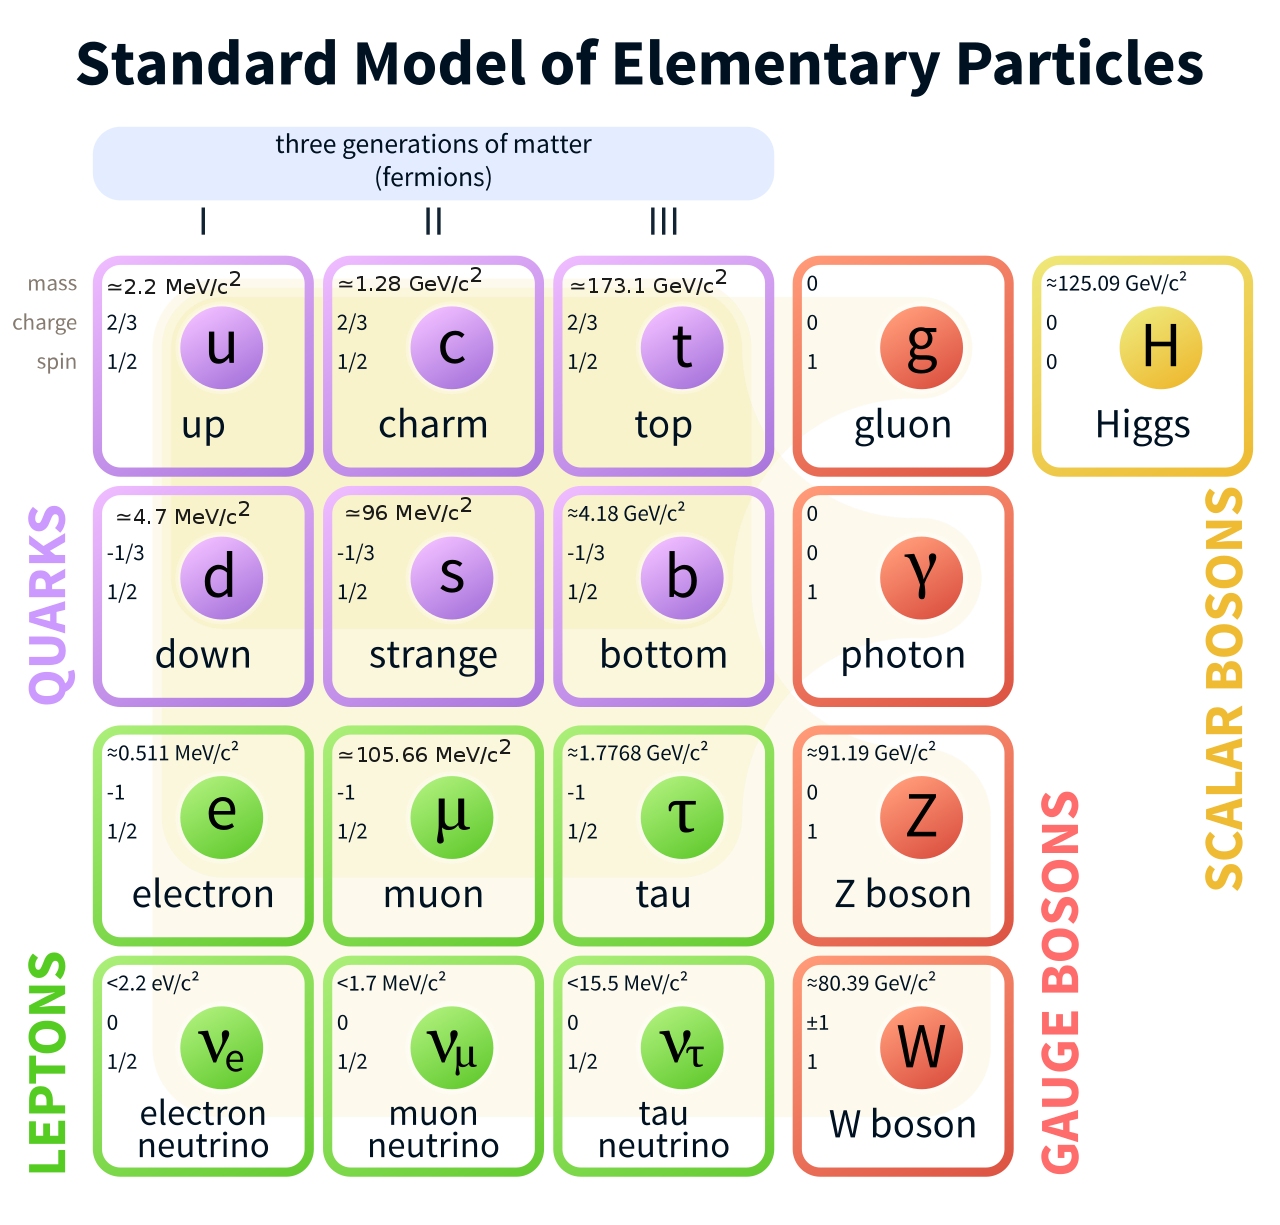
\includegraphics[width=0.9\textwidth]{figures/Chapter1/ChartOfParticles.png}
  \caption{
    The experimentally established particle content of the universe.
  }
 \label{fig:theparticles}
\end{figure}

The currently known particle content of the universe is depicted in Fig.~\ref{fig:theparticles}.
The quarks, highlighted in green, and leptons, highlighted in purple,
form matter, while the vector bosons, highlighted in red, mediate the 
interactions of this matter. The Higgs particle, shown in yellow,
has a unique role in the SM. It arises from the Higgs field, which
leads to masses for the W and Z bosons as well as the quarks and leptons.
The underlying mathematical framework used to understand the quantum 
properties of these particles and their interactions will be further discussed
in Chapter~2. 

\textbf{Go ahead and expand the description of what the particles are in this section}.

\section{Particle collider experiments}
\textbf{Introduce idea of scattering experiment}

\begin{figure}[htbp]
  \centering
   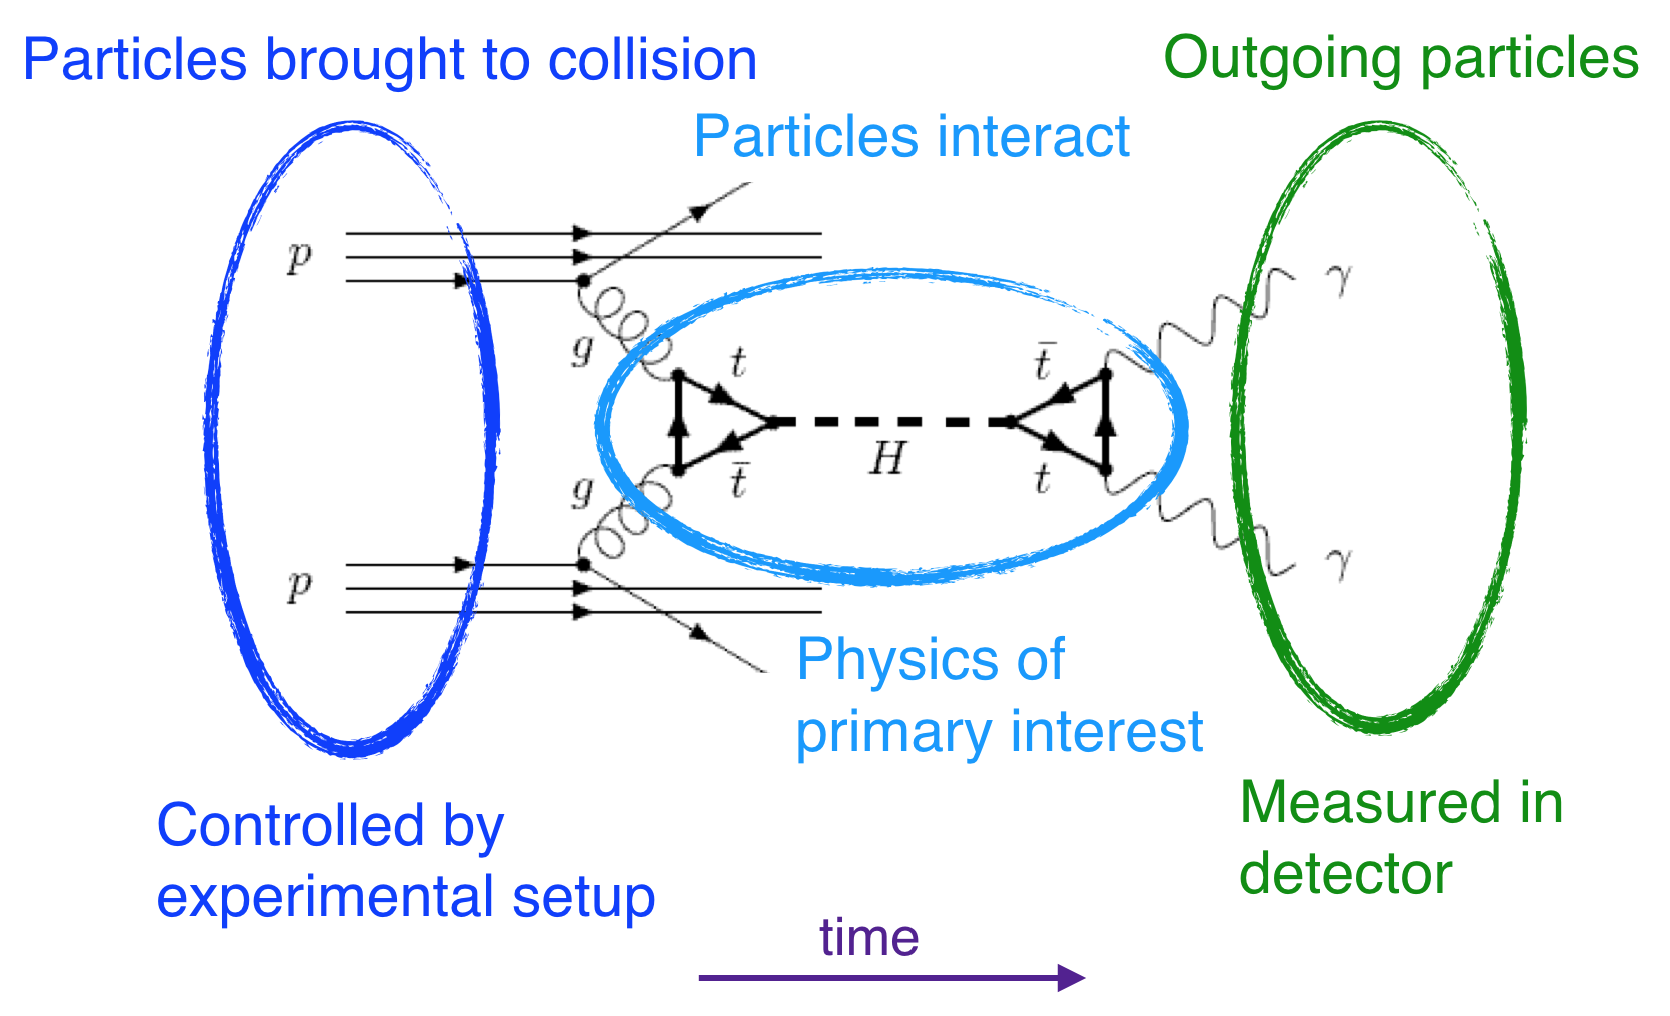
\includegraphics[width=0.9\textwidth]{figures/Chapter1/ScatteringExperiment.png}
  \caption{
  }
 \label{fig:scattering}
\end{figure}

\textbf{Introduce idea of cross section}

To observe the smallest pieces of matter, one must break matter into pieces.
The discovery of radioactivity in the late 1800s by Henri Becquerel had
profound implications for this idea, as it represented the spontaneous
disintegration of atoms. 
In addition to studying the products of these decays themselves, 
Earnest Rutherford realized the energetic decay products could be used
to perform the first particle scattering experiments. By directing the 
helium nuclei emitted from radioactive radium decay towards gold foil
and measuring the deflection
angles, he and his collaborators established the existence of the atomic nuclei.
Inferring information about the properties and interactions of particles based on their
behaviour when scattered is still central to particle physics experiment today.

Rutherford continued to use the radioactive decays of elements as a means
for particle acceleration in the early 1900s. Yet it was clear that
a means of accelerating collisions to higher energies would be needed
to continue to probe the structure of the nucleus.
These efforst lead to the invention of the 
the first particle accelerators, which have come to define the field ever since.
An electrostatic accelerator was developed at the Cavendish Laboratory
in Cambridge, England by John Crockhoff and Ernest Walton and
was used to split Lithium into Helium atoms in 1932.
Concurrently, Ernest Lawrence developed the cyclotron in California,
which became a model for many future accelerator facilities.

These inventions triggered an explosion in the field, marked by a continual 
effort to collide particles at higher and higher energies. Many major discoveries
are closely linked with technological advancements or collaborative
efforts leading to more powerful accelerators.
The facilities at the European Center for Nuclear
Research (CERN), DESY, and at the 
Fermi National Accelerator Laboratory (Fermilab) in Illinois
are strongly associated with the 
discoveries they enabled, including evidence for the force carries
of the EW and QCD interactions, the W and Z bosons and the gluon.

The most powerful collider ever built, the LHC at CERN,
now allows the study of the most energetic particle collisions ever
recorded in the laboratory, reaching concentrated energies only replicated
in the most cataclysmic events in the universe. The LHC
was planned, developed, and built over the course of decades, with
personnel and funding from countries throughout the world.
This work is based on studies of pp collisions delivered by the LHC 
and collected by the Compact Muon Solenoid detector in 2016.

\textbf{Maybe explain a bit more what a scattering experiment is here}

The LHC and Compact Muon Solenoid detector are discussed in detail 
in Chapter~3 of this thesis.

\section{Motivation and context of this result}
The work presented in this thesis
has two related motivations: performing a measurement of a rare
process predicted by the SM, and searching for signs of 
BSM physics in a channel and topology sensitive to modifications of
the EW sector of the SM.
Characterizing the self-interactions of the vector bosons is an important
step to understanding the self-consistency of the SM, and a useful probe
of possible deviations from its predictions. Because the production of events
with multiple vector bosons in the final state
requires collisions with a high center of mass energy, the LHC has
the potential to explore these states in more depth 
than previously achieved.

\begin{figure}[htbp]
  \centering
   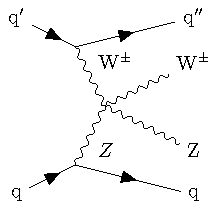
\includegraphics[page=1,width=0.25\textwidth]{figures/FeynmanDiagrams/feynmanVBS.pdf}
   \includegraphics[page=2,width=0.25\textwidth]{figures/FeynmanDiagrams/feynmanVBS.pdf}
   \includegraphics[page=3,width=0.25\textwidth]{figures/FeynmanDiagrams/feynmanVBS.pdf}
  \caption{Representative Feynman diagrams for \WZjj production in the SM and BSM. 
  EW-induced WZ production includes quartic interactions (a) of the vector bosons.
  New physics in the EW sector modifying the quartic coupling 
  can be parameterized in terms of dimension-eight effective field theory operators (b).
  Specific models modifying this interaction include those predicting charged Higgs bosons (c).
  }
 \label{fig:feynmanDiagrams}
\end{figure}

\section{Overview}

The outline of this work is as follows: Chapter~2 presents an extended 
overview of the theoretical underpinnings of this work, including the foundations
of the SM and the role of \EWWZ production in this framework. The motivations 
and structure of SM extensions probed in this work are also introduced.
Chapter~3 introduces the experimental setup and apparatus used to study W and 
Z boson production in the laboratory. The LHC and the Compact Muon Solenoid 
detector are presented and discussed. Chapter~4 describes the procedure of 
building predictions for vector boson production in pp collisions.
The use of these predictions in interpreting results, and in developing simulation
of particle production and decays in pp collisions including their interactions
with the detector -- which are used 
guide the analysis approach and optimizations -- are discussed. Chapter~5 presents
the process of finding particle candidates from electronic signals in the detector.
Chapter~6 details the procedure of this analysis and the statistical underpinnings
used to extract results. Chapter~7 discusses the results obtained from this study
including interpretations and implications. Chapter~8 summarizes the
results presented and discusses future extensions.
